\part{Fejlesztői dokumentáció}

\section{Felhasznált technológiák}

\subsection{Eclipse}
A szakdolgozatom eclipse Mars \cite{eclipse_mars} fejlesztőkörnyezetben írtam, amelyhez a quick search \cite{quick_search} nevű plugint is letöltöttem. A fejlesztést nagy mértékben megkönnyítette a fejlesztőkörnyezet használata, ugyanis többek között szintaktikus ellenőrzést, classpath ellenőrzést és ... végzett. Továbbá remekül testreszabható a ``keymapping''-je, és rengeteg hasznos billentyű kombinációt használhatunk (pl. típushierarchia, típus keresés, resource keresés, stb.).

\subsection{Maven}
A népszerű buildrendszerből a 3.3.3-as verziót használtam, amelyhez igen sok különböző plugin szerezhető be. Eredetileg csupán a függőségek kezelésére alkalmaztam volna a programot, később egyre több és több pluginnal egészítettem ki, így egyre több feladatot volt képes ellátni a szoftver.

\subsubsection{Adatbázis ``húzás''}
Az adatbázist a fejlesztés elején kézzel húztam újra, majd rátaláltam a sql-maven-plugin nevezetű pluginra. A maven oldalán megtalálható teljeskörű dokumentáció segítségével bekonfiguráltam a plugint, így csupán a
 \begin{verbatim}
mvn sql:execute@create-db
mvn sql:execute@create-triggers
mvn sql:execute@fill-db
\end{verbatim}
utasításokat kellett kiadnom parancssorból, hogy friss adatbázissal dolgozhassam tovább. Igyekeztem a felesleges parancsismétléseket eliminálni, vagyis letöltöttem az exec-maven-plugin nevű plugint, amelynek segítségével sikerült a 
 \begin{verbatim}
mvn exec:exec
\end{verbatim}
parancsra korlátozni az adatbázis újrahúzását. Próbáltam tovább absztrahálni a feladatot, majd végül egy profilt készítettem el, amely az install fázissal együtt oldja meg az adatbázis kérdést. A 
 \begin{verbatim}
 mvn clean install -Pbootstrap
 \end{verbatim}
parannccsal nem csak a lokális repozitorinkba telepíthetjük fel a poker-persist modult, de még egy új adatbázist is kapunk.

\subsubsection{Javadoc}
A mavennel java dokumentációt is lehet generáltatni a
\begin{verbatim}
 mvn javadoc:javadoc
\end{verbatim}
 parancs segítségével. Sőt, akár modul dokumentációt is lehet készíteni a 
\begin{verbatim}
 mvn site:site
 mvn site:stage
\end{verbatim}
utasításokkal. Az elkészült dokumentációk a modul \path{modul\target\staging} könyvtárba kerülnek. Kettő darab index.html állományt kell keresnünk, az egyik a gyökérkönyvtárban található a másik pedig az \path{apidocs} könyvtár gyökerében.
 
\subsection{MySQL}
\subsection{Git}
A fejlesztés során előfordult, hogy internet kapcsolat nélkül kellett verzióznom a kódomat. A git egyik legnagyobb előnye, hogy internet kapcsolat nélkül is lehet commit parancsot végrehajtani. A commit parancs hatására a lokális repozitorinkba egy új snapshot (pillanatfelvétel) készül a working directory tartalmáról, amelyet később push utasítással feltölthetünk egy távoli repozitoriba. A fejlesztéshez több branchet is használtam, így ha valami balul sült volna el, akkor egyszerűen visszaálltam volna a masterre.

\subsection{Enterprise Architect}
A tervezés során igen nagy hasznát vettem ennek a szoftvernek. Rengeteg beállítás, funkció megtalálható a programban. Szinten minden testreszabható a segítségével. Az elkészült UML diagramokból pedig JAVA kódot tud generálni a program. A dokumentációban fellelhető osztály hiearchiák és UML diagramok ennek a szoftvernek a segítségével készültek el.

\section{Adatbázis séma}
\begin{figure}[h!]
  \caption{Adatbázis séma}
  \centering
    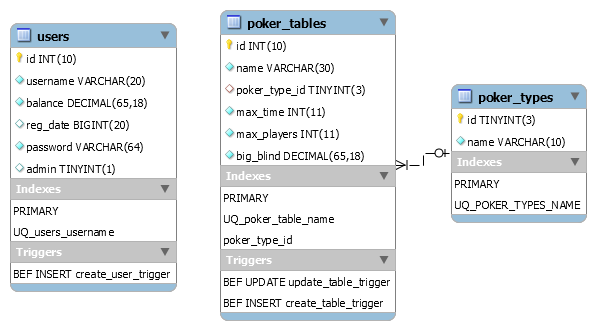
\includegraphics[width=\textwidth]{user-documentation/images/db_scheme.png}
\end{figure}
Az adatbázis (ld. X. ábra) 3 táblából épül fel
\begin{itemize}[leftmargin=2.7cm]
\item users
\item poker\_tables
\item poker\_types
\end{itemize}
 Minden tábla rendelkezik elsődleges kulcssal, amelynek típusa UNSIGNED INTEGER, kivétel a poker\_types táblát, ugyanis ennek a táblának az elsődleges kulcsa UNSIGNED TINYINT típusú, amelyet a MySQL Server 4 byteon tárol. Az adatábrázolás mértékének a szűkítése ebben az esetben indokolt, ugyanis a 255 különböző értékű UNSIGNED TINYINT típus kielégíti a játéktípusok által támasztott követelményeket. A játékstílusok neveit is el kell tárolni, amelynek a maximális hossza 10 karakterben lett meghatározva, amely triggerrel van védve. A users tábla tartalmazza a regisztrált felhasználókat. A regisztrált felhasználók felhasználónévvel és jelszó párossal tudnak regisztrálni, és ennek megfelelően ezek az adatok tárolásra is kerülnek. A felhasználónév maximális hossza 20 karakter, ameyelet triggerrel ellenőrzök. A jelszót bcrypt függvénnyel nyírom. Só eltárolása nem szükséges a bcrypt implementációjából adódóan. A felhasználóról el kell még tárolni a regisztráció dátumat, amely a szerver ideje alapján számolódik és UNIX timestampként kerül letárolásra, továbbá a jogosultsági (admin) szintet, amely ugyancsak 4 byteon (TINYINT) kerül ábrázolásra. A 0/1 értékek megfeleltethetőek a TRUE/FALSE logikai típusú konstans értékeknek, így tehát, ha az érték 0, vagyis FALSE, akkor az adott felhasználó nem rendelkezik admin jogkörrel, különben igen. Ugyancsak tárolandó érték a felhasználó játékbeli egyenlege, amely BIGDECIMAL típúsként van ábrázolva.
A játéktáblákat a poker\_tables adatbázis tábla tárolja. Szükségünk van eltárolni a játéktábla nevét, melynek felső korlátja 30 karakter és egyedinek kell lennie. Ezeket a megszorításokat szintén triggerekkel ellenőrzöm. A játék asztal játékstílusát is eltárolom, amely egyben idegenkulcs is a poker\_types táblára nézve. Továbbá minden asztal tulajdonsága, hogy maximum hányan játszhatnak rajta, és hány másodpercig gondolkodhatnak a játékosok. Ezen két érték típusaként ugyancsak UNSIGNED TINYINT van meghatározva, ugyanis az egyes asztaloknál a játékosok száma legfeljebb 5 lehet, míg az egyes játékosok gondolkodási ideje maximum 40, de legalább 5 másodperc.

\section{Megoldási terv}
\subsection{Probléma}
\subsection{Tervezés}
\subsection{Implementálás}
\subsection{Elemzés}

\section{Modulok}
A programcsomag 6 fő modult tartalmaz
\begin{description}
  \item[poker-server] \hfill \\
  A póker játék szervere, amely magát a játékot szolgáltatja.
  \item[poker-client] \hfill \\
  A póker játék kliense, amely segítségével a szerverhez lehet csatlakozni.
  \item[poker-shared] \hfill \\
   A póker játék azon modulja, amelytől a szerver és a kliens egyaránt függ.
   \item[poker-persist] \hfill \\
   Az adatok letárolásáért felelős modul.
   \item[poker-model] \hfill \\
   A póker játék modellezéséért felelős csomag.
   \item[javapokertexasholdem] \hfill \\
   Külső könyvtár, amely a nyertes játékos kiértékelési feladatot végzi.
\end{description}
\begin{figure}[h!]
	\caption{Kliens modulra bontása}
	\label{fig:client_modul}
	\centering
	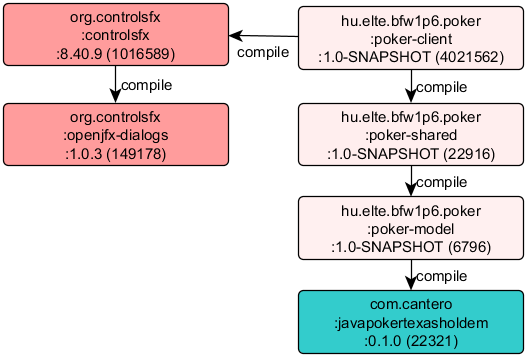
\includegraphics{user-documentation/images/poker-client-deps.png}
\end{figure}
\begin{figure}[h!]
	\caption{Szerver modulra bontása}
	\label{fig:server_modul}
	\centering
	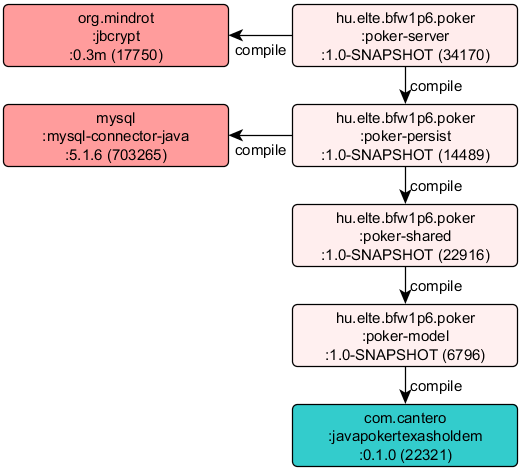
\includegraphics{user-documentation/images/poker-server-deps.png}
\end{figure}
A modulok közötti függőséget a \ref{fig:client_modul}. és a \ref{fig:server_modul}. ábra szemlélteti. \\
A programcsomag két főmodulra bontható
\begin{itemize}[leftmargin=2.7cm]
\item poker-server
\item poker-client
\end{itemize}

\subsection{Model} \label{sec:poker-model}
A poker-model modul felelős a játék modellezésért. A X. ábrán látható a modul felépítése. Az entitásokat össze kellett fogni az EntityWithId interfész segítségével, ezáltal a DAO (későbbi képre hivatkozás...?) objektumot generikusan lehetett megfogalmazni, amely segített a kód duplikációk elkerülésében. A PokerTable és a User osztályok példányai feleltethetőek meg a poker\_tables és a users adattáblák egyes rekordjainak. A PokerType enumeráció a játékstílusokat határozza meg. Ha egy új játékstílust szeretnénk hozzáadni a játékhoz, akkor a kódban egy új PokerType enum objektumot kell felvennünk, és a poker\_schema.sql állományban pedig fel kell venni egy új insert utasítást a poker\_types táblára nézve az új játékstílus nevére vonatkozólag. Természetesen ez a pár sor újonnan hozzáadott kód nem azt jelenti, hogy már használhatjuk is az új játékstílust. A programcsomagot több ponton is ki kell bővíteni
\begin{itemize}[leftmargin=2cm]
	\item Szerver oldal
		\begin{enumerate}
			\item AbstractPokerTableServer osztályt ki kell terjeszteni egy új osztállyal
		\end{enumerate}
	\item Kliens oldal
		\begin{enumerate}
			\item Új leszármazott osztályokat kell létrehozni a kliens oldali MVC absztrakciós osztályaiból (ld. később) vagy hivatkozva...
			\item Új fxml állományt kell létrehozni
		\end{enumerate}
\end{itemize}

\subsection{Shared}
A poker-shared modul olyan közös osztályokat tartalmaz, amelyeket a kliens és a szerver egyaránt használ. Itt helyezkednek el az egyéni kivételek, a kommunikációs rendszer definíciója és a kliens, mint megfigyelő interfésze.

\subsubsection{Kivételek}
A játékcsomagnak szüksége van egyéni kivételekre. Az olyan speciális eseteket, mint például adabázisba írás, illetve abból olvasás közbeni fellépő kivételt saját kivételobjektumokkal célszerű lekezelni. Ehhez hasonló egyéni kivételek fellépthetnek bejelentkezéskor, asztalhoz való csatlakozáskor, hibás jelszó megadás esetén, stb (ld. melléklet, javadoc...).

\subsubsection{Kommunikációs rendszer}
A szerver és a kliens  üzeneteket küldhetnek egymásnak. \\
Ide jöhet a kép... Az ún. messaging systemet igyekeztem minél absztraktabb módon megfogalmazni, ezzel is elősegítve a későbbi bővíthetőségi nehézségeket. Azonban sajnos helyenként fellelhető kód duplikáció az enumerációkra való építkezés miatt. \\
Minden utasításnak kötelezően implementálnia kell a PokerCommand interfészt, ezzel is elősegítve az általános megfogalmazást a rendszerben. Két fajta utasítás létezik a játékcsomagban:
\begin{itemize}[leftmargin=2cm]
	\item Szerver utasítás
	\item Kliens utasítás
\end{itemize}
Továbbá a játékstílusnak megfelelően tovább szigorodik... (kéne egy jó szó) a küldendő üzenet fajtája. A programcsomag kettő játékstílust fogalmaz meg (ld. \ref{subsubsec:game_styles}). A játékstílusok különböző utasítás fajtákat igényelnek. Értelemszerűen, ha egy Holdem játékstílusban résztvevő kliens üzenetet szeretne küldeni a játék asztal szervernek , akkor egy HoldemPlayerCommand típusú objektumot kell elküldenie a szerver csonkon keresztül. \\
Az üzeneteknek vannak fajtái, amelyeket a mellékletben meg lehet tekinteni.

\subsubsection{Observer pattern \cite{observer_pattern}}
Az oberserver tervezési minta segítségével megvalósítható RMI API-n keresztül az ún. event driven server. Így nem csak a kliens tud üzenet küldeni a szervernek, hanem a szerver is tudja értesíteni a klienseket. Például, ha egy játékos CHECK típusú utasítást küldött a szervernek (játékstílustól függetlenül), akkor azt az üzentet a szerver minden kliensnek szétszórja (broadcast, üzenetszórás... valahogy jól kéne megfogalmazni).

\subsubsection{Session}
% ez a szöveg lehet, hogy server modulba kéne....
A szerver a klienseket session objektumokkal azonosítja. Minden kliens kap egy sessiont a bejelentkezéskor. A session addig él, amíg a felhasználó ki nem jelentkezik, akkor ugyanis a munkamenet érvénytelenítésre kerül. Illetőleg a munkamenetet akkor is érvényteleníteni kell, ha a kliens nem jelentkezett ki, de a kapcsolat valamilyen oknál fogva megszakadt. \\
Amikor egy kliens be szeretne jelentkezni a játékba, akkor a szerver az összes megszakadt kapcsolatú klienst felderíti, és a munkamenetüket érvénytelennek tekinti. A felderítés ún. pingeléssel történik. A szerver minden csatlakozott klienst megpróbál elérni, és amelyik kliensnél megszakadt a kapcsolat, azt eltávolítja a szerverről. Ezután a SessionService ellenőrzi, hogy az adott felhasználónévvel van-e aktív munkamenet, ha van, akkor kivételt dob az eljárás, különben az autentikáció sikeres, és a kliens oldali model eltárolja a loginkor kapott sessiont.

\subsection{Persist}
A poker-persist modul látja el az adatbázissal kapcsolatos teendőket. Ez a modul írja és olvassa az adatbázist a bejövő kérések és paraméterek alapján.

\subsubsection{Generikus DAO}
A generikusság elengedhetett a kódismétlés elkerülése végett. Általánosan kell megfogalmazni az entitások viselkedését \ref{sec:poker-model} (vagy fordítva...), és ezáltal a persist modul letisztult arculatot kap. A GenericDAO osztály tartalmaz minden olyan elemet, amelykre a specializálódott DAO-knak szükségük lehet.

\subsubsection{Adatbázis menedzser}
Az AbstractDAO-nak szükséges van tényleges adatbázis kapcsolatra, amelyet a DBManager osztály szolgáltat.

\subsubsection{Kivételek átfordítása}
Az AbstractDAO rendelkezik egy SQLExceptionTranslator objektummal is, amely az adatbázisból érkező hibát fordítja át PokerDataBaseException típusú kivételre. A PokerDataBaseException kivétel osztály a felhasználó számára is értelmes hibaszöveget hordoz magában.

\subsection{Kliens}
A kliens modult és annak minden függőségét egy jar fileba csomagolva kell szétterjeszteni a felhasználók között, akik majd ténylegesen használni fogják a programot. A \ref{fig:client_modul}. ábra alapján a jar file tartalmazni fog minden olyan osztályt és interfészt, amelyre ténylegesen szüksége lesz a kliens programnak. Az összecsomagoláshoz igénybe vehetjük a mavent és annak az assembly pluginját. A poker-client könyvtárban a
 \begin{verbatim}
mvn clean compile assembly:single
\end{verbatim}
paranccsot kiadva a poker-parent/release könyvtár alá csomagolódik be a futtatható jar állomány. \\
\subsubsection{Model-View-Controller \cite{MVC}}
Az igen közkedvelt tervezési minta alapján valósítottam meg a kliens oldali programot.

\pokerparagraph{Model}
A kliens kettő darab model osztályt tartalmaz. Az Model nevű singleton osztály felelős a szerver felé irányuló kapcsolat kiépítésében és fenntartásában. Ez az egyszerű szerver hívásokat végzi el. A kliens indulásakor elkéri a registry-ből a szerver csonkot, és bejelentkezéskor eltárolja a szerver által generált munkamenet objektumot. A model segítségével hívhatóak meg a játék funkcióinak a zöme. Ide sorolható a játék minden olyan funkciója, amely nem játék asztalhoz köthető. Például ennek a modelnek a segítségével lehet bejelentkezni, asztalt és felhasználót módosítani, vagy akár a játékasztalokat elkérni a szervertől. \\
A kliens tartalmaz egy másik modelt - AbstractMainGameModel -, amely a tényleges játékért felel kliens oldalon. A szerver a parti megkezdésekor leküldi a klienseknek, hogy az adott partiban ki hol ül az asztalnál, hány játékos ül az asztalnál, a játékosok neveit és még néhány inicializációs értéket. Ezen értékek alapján a model el tudja dönteni, hogy az adott kliensnek kötelezően be kell rakni vakot. Minden parti elején minden kliensnek az adóssága a nagy vakkal egyezik meg. A további körökben az adósság leróható.

\pokerparagraph{View}
A megjelenítésért a JavaFX 2 \cite{javafx} felel. Az alapkonstrukció, hogy a GUI-n megjelenő objektumok zömét fxml állományokba szervezzük és a megjelenítés színtérgráffal történik. Minden fxml állományhoz pontosan egy controller tartozik, amely az fxml állomány minden újratöltésekor inicializálódik. A controllert az adott fxml állomány gyökerébe kell bekötni. \\
A programcsomag által definiált játékstílusok igen hasonlóak, ezért egy AbstractMainView osztályban megfelelően kiszervezhetőek a közös részek, majd ennek az osztálynak a specializációiban (ClassicMainView, HoldemMainView) kerülnek megvalósításra a tényleges játékstílusbeli különbségek. Például eltérő különbség , amely a GUI-n is megjelenik, hogy a játékosok hány darab kártyalapot kapnak kézbe, illetve a Texas Hold'Em játékstílussal ellentétben a classic játékmódban nincsenek közös kártyalapok.

\pokerparagraph{Controller}
A controller általános szerepét ugyancsak egy abstract osztály, az AbstractMainGameController tölti be. A közös részek nem csak a megjelenítés és a model szintjén figyelhetőek meg, hanem az őket összekötő controller szintjén is. A beérkező utasítások alapján a controller hív tovább a megjelenítési és a model rétegbe.

\subsubsection{Communication controller}


\subsubsection{PokerRemoteObserver}


\subsubsection{FrameController}

\subsection{Szerver}
\begin{figure}[h!]
  \caption{A szerver publikus interfésze}
  \label{fig:server_public}
  \centering
    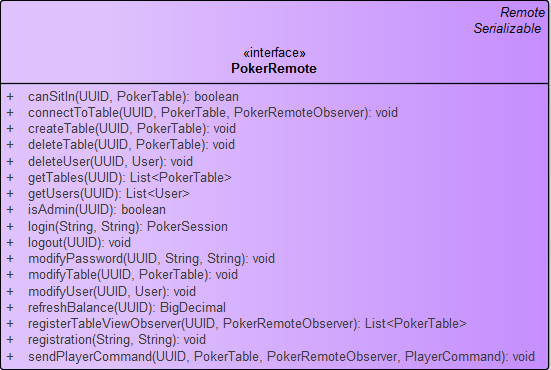
\includegraphics[width=\textwidth]{user-documentation/images/server_remote.png}
\end{figure}
A szerver feladata a játék biztosítása a kliensek számára. A \ref{fig:server_public}. ábrán látható a szerver jóldefiniált publikus interfésze. A kliensek ezt az interfészt tudják elkérni a registry-ből \cite{RMI}. A PokerRemote interfészt a PokerRemoteImpl osztály implementálja, ennek egy instanciája a tényleges szerver objektum. A szerveren futnak a játékasztal-szerverek, amelyek egy-egy asztalnak feleltethetőek meg, amelyekhez a kliensek csatlakozni tudnak. Ha egy játékos csatlakozik egy játékasztalhoz, akkor az adott asztal feljegyzi a csatlakozott klienst egy lokális listába. A főszervernek továbbra is van referenciája a klienshez, ugyanis minden klienstől érkező utasítást a főszerver fogad, és irányít a megfelelő játékasztal-szerverhez. Erre az autentikáció miatt van szükség. Azonban ez a fajta megközelítés könnyen szűk keresztmetszetté válhat, hiszen (vagy ezt inkább tovább fejlesztési lehetőségek...) \\
A szerver a jelszavak titkosítására bcrypt eljárást alkalmaz, amelynek a biztonságát sózással növeli. Továbbá a szerver felhasznál még egy külső csomagot - mysql-connector-java -, amely az adatbázis kapcsolatért felel.

\subsection{javapokertexasholdem}
Külső könyvtár, amely eredetileg Texas Hold'Em játékstílusban tud kezeket kiértékelni. Az integrációt viszonylag könnyen meg lehetett oldani, ráadásul még általánosítani is sikerült a könyvtárat. Tehát classic és Texas Hold'Em játékstílusra is ugyanezt a könyvtárat használja a szerver a kezek kiértékelésére.

\section{Funkciók}
A szerver vázáért a PokerRemote interfész felel, amely a játékon végrehajtható műveletek összefogásáért felel. Itt található az összes funkció, amely megvalósításra került, mint például játék asztal létrehozása, új felhasználó létrehozás, admin jog kiosztása stb. A kliens ezt a vázat tudja elkérni az RMI registry-ből, mint kliens-oldali szervercsonk, amelyeken a műveletek meg tudja hívni.
\subsection{Általános funkciók}

\subsubsection{Regisztráció}
A játékot csak regisztrált felhasználók tudják használni. A szerver biztosít regisztrációs lehetőséget a felhasználók számára. A regisztráció során felhasználónevet és jelszót köteles megadni a felhasználó, amely tárolásra kerül az adatbázisban. Minden újonnan regisztrált felhasználó 1000 egységnyi egyenleggel rendelkezik. Az adatbázis séma nem engedi, hogy több azonos felhasználónévvel különböző felhasználók regisztrálva legyenek, erre a regisztráció során ügyelnie kell a felhasználónak.

\subsubsection{Bejelentkezés}
A játék használatához a játékosoknak be kell jelentkezniük. Egy felhasználónévvel egyidőben csak egy munkamenet létezhet. Ha a felhasználó már használatban lévő felhasználónévvel kíván beljelentkezni, akkor a szerver hibás bejelentkezési adatokra hivatkozva megtagadja az utasítást. Sikeres bejelentkezést követően a szerver példányosít egy PokerSerssion objektumot egy UUID \cite{uuid} azonosítóval, amelyet lokálisan eltárol, majd a kliensnek elküld. A kliens a kijelentkezésig megőrzi ezt az objektumot, és a későbbi funkciók hívása során ezzel a munkamenettel azonosítja magát.

\subsubsection{Kijelentkezés}
A játékosok a kijelentkezés funkcióval hagyhatják el a játékot. A funkció hivása során a kijelentkezni kívánó felhaszáló munkamenetét a szerver érvényteleníti, és a felhasználó visszakerül a bejelentkezési formhoz. A szerver (korlátozott mértékben) fel lett készítve a nem szabályszerű kijelentkezésre, tehát ha például megszakad a kapcsolat a klienssel, akkor a legközelebbi bejelentkezési funkció hívása során a szerver érvényteleníti a megszakadt kliensek munkameneteit, ezzel elérve azt, hogy a foglalt felhasználónevekkel újra be lehessen jelentkezni.

\subsubsection{Asztalok}
\pokerparagraph{Létrehozás}
A funkció eléréséhez admin jogosultságra van szükség. Egy új asztalt lehet lérehozni az adatbázis séma (hivatkozás) irányelvei szerint megfelelően paraméterezve. Amikor a kliens asztalt szeretne létrehozni, akkor a szerver egyértelműen tájékoztatja, hogy az asztal létrehozás sikeres volt-e. Ha igen, akkor egy felugró üzenet jelenik meg a képernyőn, hogy az asztal létrehozása sikeres volt, majd a felhasználó vissza lesz irányítva a tábla listázó felületre. Ha az asztal létrehozása sikertelen volt, akkor a felület ugyancsak egyértelműen jelzi a felhasználónak, hogy a művelet miért hiúsult meg. Például előfordulhat hibás beviteli érték, szerverhiba és adatbázishiba is.

\pokerparagraph{Módosítás}
Egy már meglévő asztalt adminisztrációs joggal rendelkező felhasználó módosíthat. Fontos megjegyezni, hogy a módosítás csak üres asztalokra alkalmazható.
\pokerparagraph{Törlés}
A funkcióhoz ismételten adminisztrációs jog szükséges. Már létező asztal törölhető a funkció segítségével. A funkciót csak üres asztalokra lehet alkalamazni.
\pokerparagraph{Lekérés}
A bejelentkezést követően a felhasználó a táblalistázó felületre kerül, ahol megtekintheti a létrehozott és elindított játéktábla-szervereket (hivatkozás). A bejelentkezést követően a kliens ezeket az asztalokat elkéri a szervertől. Fontos megjegyezni, hogy ha bármelyik asztal módosításra került, akkor az asztalokat a szerver újra leküldi a klienseknek, így minden kliensnél az asztalok legfrissebb változata lesz elérhető.

\pokerparagraph{Csatlakozás}
A felhasználók létrehozott játékasztal-szerverekhez csatlakozhatnak. Fontos megjegyezni, hogy egy asztalnál maximum 5 játékos ülhet egyszerre, tehát ha egy asztal tele van (5 játékos ül az asztalnál, beleszámolva a következő partira váró játékosokat is), akkor kliens oldali kód nem engedi beülni a felhasználót az adott asztalhoz, amelyről a felhasználót a képernyőn értesíti. Ha egy tele asztaltól kilép az egyik játékos (vagy megszakad a kommunikáció), akkor az asztalnál felszabadul egy hely, amelyet egy új felhasználó elfoglalhat, ekkor az asztal ismét tele lesz.

\pokerparagraph{Szabad helyek lekérdezése}
Ha egy kliens be szeretne ülni az egyik játékasztal-szerverhez, akkor előbb le kell kérdeznie, hogy van-e még szabad hely az asztalnál.

\subsubsection{Felhasználók}
\pokerparagraph{Létrehozás}
A regisztráció során új felhasználó entitás jön létre, amelyet a szerver letárol az adatbázisban. A funkció külön, direktbe nem hívható, regisztrációhoz kötött.

\pokerparagraph{Módosítás}
\pokerparagraph{Törlés}
\pokerparagraph{Lekérés}
\pokerparagraph{Jelszó csere}
A felhasználóknak lehetőségük van jelszócserére

\pokerparagraph{Adminisztrációs jog}
A szerverre beregisztrált felhasználók alapesetben nem rendelkeznek ilyen jogosultsággal. Az adminisztrációs jogot csak adminisztrációs joggal rendelkező felhasználó tudja kiosztani illetve megvonni. Friss adatbázis esetén létezik egy admin nevű felhasználó, aki adminisztrációs joggal rendelkezik. Kezdetben csak ez a felhasználó tud kiosztani adminisztrációs jogot.

\subsection{Játékmenetbeli funkciók}
\subsubsection{Utasítás küldés}
\subsubsection{Egyenleg lekérése}

\section{Tovább fejlesztési lehetőségek}
\begin{itemize}
\item Az adatbázis viszonylag alacsony absztrakciós szinten került implementására, azonban mivel néhány tábláról beszélhetünk csak, ezért igyekeztem elkerülni a keretrendszerek általi overheadet. Ugyanakkor ezen a ponton sokat fejlődhet a programcsomag, ha a későbbiek során esetlegesen bonyolultabban kellene modellezni a játékot adatbázis szempontjából. Például dialektusok - akár Liquibase (hivatkozás) - használata elfedheti a tényleges adatbázis-kezelő rendszer általánosságait, így eggyel magasabb szintre helyezhető a megvalósítás.
\item A felhasználói élményen sokat javíthat az animációk használata. A megjelenítés sokkal lágyabb, folyékonyabb lehetne Transition/Animation (bibliográfiába hivatkozás...) objektumok használatával.
\item Akár a komplett RMI architektúrát le lehetne váltani, és helyette REST szoftverarchitektúrát alkalmazni, amely modernebb megjelenést (AngularJS, reszponzív design) és modernebb fejlesztői eszközöket, API-kat vonna maga után.
\item A játék nem képes kezelni olyan eseteket, amikor egynél több játékos nyer az adott körben.
\item A játék nincs felkészítve arra a szélsőséges esetre, ha valakinek elfogy a zsetonja, akkor pontosan minek (és hogyan) kell történnie.
\item A kódban viszonylag sok kód duplikáció van jelen, ugyanis az HouseCommandType és a PlayerCommandType enum típusú objektumok szűk keresztmetszetnek tudható be. Ha a PokerCommand interfacet implementáló osztályokat generikusan tudnánk megfogalmazni, akkor jelentősen letisztulna a kód.
\item Az admin jogot el lehetne távolítani a játékból, és helyette MVC tervezési minta alapján a szerver oldalra is implementálni lehetne egy grafikus interfészt, amelyen keresztül a szerver teljeskörű karbantartása és adminisztrációja elvégezhető lenne.
\end{itemize}

\section{Tesztelés}
\subsection{Funkcionális tesztelés}
%\begin{tabulary}{| K{2cm} | K{2cm} | K{2cm} |}
%\hline
%  Funkció & Elvárt eredmény & Eredmény \\ \hline
%  Regisztráció & A felhasználó a regisztrációt követően be tudjon jelentkezni a póker játékba. & A program jelezte a felhasználónak, hogy a regisztráció sikeresen megtörtént, és visszairányította őt a bejelentkezési formhoz, amelyet értelemszerűen kitöltve be tudott jelentkezni. \\ \hline
%  Bejelentkezés & A formot helyesen kitöltve a program sikeresen autentikálta és beléptette a felhasználót. & Regisztrációt követően be tudjon jelentkezni a felhasználó \\ \hline
%  Tábla módosítás & - & - \\ \hline
%  Tábla törlés & - & - \\ \hline
%\end{tabulary}


\clearpage
